\documentclass[12pt]{article}

% Idioma e codificação
\usepackage[brazil]{babel}
\usepackage[utf8]{inputenc}
\usepackage[T1]{fontenc}

% Matemática e listas
\usepackage{amsmath, amssymb}
\usepackage{enumitem}

% Layout e cores
\usepackage{geometry}
\usepackage{graphicx}
\usepackage{xcolor}
\usepackage{url}
\usepackage{listings}
\usepackage{booktabs}
\usepackage{subcaption}

% TikZ para prototipagem de telas e diagramas
\usepackage{tikz}
\usetikzlibrary{shapes.geometric, arrows.meta, positioning, calc, fit, backgrounds, shadows}

% Cores institucionais e tema do App
\definecolor{navyblue}{RGB}{0,0,128}
\definecolor{meuazul}{RGB}{0, 79, 151}
\definecolor{meucinza}{RGB}{80, 80, 80}
\definecolor{meuvermelhoescuro}{RGB}{180, 30, 30}
\definecolor{meuverde}{RGB}{30, 130, 60}

% Cores do Protótipo (Light Theme Visão Computacional)
\definecolor{appbg}{RGB}{240, 244, 248}
\definecolor{cardbg}{RGB}{255, 255, 255}
\definecolor{cardbglight}{RGB}{248, 250, 252}
\definecolor{cyanaccent}{RGB}{14, 165, 233}
\definecolor{cyanbtn}{RGB}{2, 132, 199}
\definecolor{textwhite}{RGB}{31, 41, 55}
\definecolor{textmuted}{RGB}{107, 114, 128}
\definecolor{bboxcolor}{RGB}{14, 165, 233}

% Configuração do Listings para JSON
\lstdefinelanguage{json}{
  basicstyle=\ttfamily\small,
  showstringspaces=false,
  breaklines=true,
  frame=single,
  backgroundcolor=\color{gray!5},
  rulecolor=\color{meucinza!40},
  stringstyle=\color{meuazul},
  keywordstyle=\color{meuvermelhoescuro}
}

% Margens
\geometry{margin=2.0cm}

% Cabeçalho e rodapé
\usepackage{fancyhdr}
\pagestyle{fancy}
\fancyhf{}

\renewcommand{\headrulewidth}{2pt}
\renewcommand{\footrulewidth}{2pt}

\renewcommand{\headrule}{\hbox to\headwidth{%
  \color{navyblue}\leaders\hrule height \headrulewidth\hfill}}

\renewcommand{\footrule}{\hbox to\headwidth{%
  \color{navyblue}\leaders\hrule height \footrulewidth\hfill}}

\setlength{\headheight}{52pt}
\addtolength{\topmargin}{-20pt}

% Cabeçalho
\fancyhead[L]{%
  
\includegraphics[height=1.2cm]{logo.png}
}

\fancyhead[R]{%
  \raggedleft
  \textcolor{navyblue}{%
    \small
    \textbf{Trabalho Prático Avaliativo — N2}\\
    Prof.~Me.~Sergio Souza Novak\\
    \textit{DESENVOLVIMENTO DE SOFTWARE PARA DISPOSITIVOS MÓVEIS}
  }
}

% Rodapé
\fancyfoot[C]{\textcolor{navyblue}{\thepage}}

% =========================
\begin{document}
% =========================

\begin{center}
    {\Large \textbf{ENUNCIADO DO TRABALHO PRÁTICO (N2)}} \\[0.2cm]
    {\large \textbf{Disciplina:} DESENVOLVIMENTO DE SOFTWARE PARA DISPOSITIVOS MÓVEIS} \\[0.1cm]
    {\small \textbf{Tema:} Aplicativo Android Full-Stack em Kotlin: Visão Computacional, Inferência On-Device e Persistência em Servidor}
\end{center}

\hrule

\vspace{0.3cm}

\section{Objetivo do Trabalho}
O objetivo deste trabalho prático é consolidar os conhecimentos adquiridos na disciplina através do desenvolvimento de uma solução computacional completa (\textbf{Full-Stack Mobile}). Os alunos deverão construir um aplicativo nativo em \textbf{Kotlin} focado em \textbf{Visão Computacional e Inferência On-Device} integrado a um \textbf{Servidor Backend} para persistência de dados e estatísticas.

Os grupos deverão definir a proposta do seu produto móvel, projetar o seu próprio \textbf{Design System} (paleta de cores, tipografia e identidade visual), escolher um dataset no \textbf{Roboflow}, integrar a inferência local off-line com modelos \textbf{YOLO / ONNX} fornecidos pelo professor e comunicar-se com um servidor backend (desenvolvido em Node.js, Python, Kotlin ou linguagem à escolha) para armazenar e consultar o histórico e os relatórios geométricos de cada análise realizada.

---

\section{Fluxo de Trabalho e Etapas do Projeto}

O desenvolvimento da solução seguirá o seguinte fluxo de trabalho entre os grupos e o professor:

\begin{enumerate}[label=\textbf{Etapa \arabic*:}]
    \item \textbf{Seleção do Dataset no Roboflow:} O grupo escolhe no \textbf{Roboflow Universe} (\url{https://universe.roboflow.com}) um dataset público rotulado de detecção de objetos adequado ao seu projeto.
    \item \textbf{Validação com o Professor:} O grupo submete a proposta e o link do dataset para aprovação do professor.
    \item \textbf{Treinamento YOLO e Entrega ONNX:} O professor realiza o treinamento da rede neural \textbf{YOLO} e disponibiliza para a equipe o modelo em formato \textbf{ONNX} (\texttt{.onnx}).
    \item \textbf{Criação do Design System do Grupo:} Os alunos elaboram a identidade visual do aplicativo (paleta de cores, tipografia, estilos de botões e cartões).
    \item \textbf{Desenvolvimento do Servidor Backend:} Construção de uma API REST (em Node.js, Python, Kotlin, etc.) com rotas para receber, persistir e retornar os relatórios de inferência em Banco de Dados (SQL/NoSQL) ou em arquivos JSON.
    \item \textbf{Desenvolvimento da Aplicação Android em Kotlin:} Construção do aplicativo móvel com inferência local off-line via ONNX Runtime, envio automático da telemetria para o servidor backend e telas de consulta ao histórico de análises.
\end{enumerate}

---

\section{Requisitos Funcionais e Arquitetura}

Os grupos deverão implementar os seguintes requisitos funcionais no aplicativo e servidor:

\begin{enumerate}[label=\textbf{RF\arabic*:}]
    \item \textbf{Gerenciamento de Modelos ONNX:} Suporte para carregar o modelo ONNX embarcado ou selecionar um arquivo \texttt{.onnx} a partir do armazenamento do dispositivo.
    \item \textbf{Aquisição de Imagens (Câmera / Galeria):} Integração funcional com a câmera nativa e com a galeria de mídia do Android.
    \item \textbf{Ajuste Dinâmico de Parâmetros:} Controle interativo com \textit{Slider} para o Limiar de Confiança (\textit{Confidence Threshold}) e filtro de rótulos/classes.
    \item \textbf{Pipeline de Inferência Local On-Device:} Execução 100\% local do modelo ONNX no hardware móvel (CPU/NPU/GPU) sem dependência de nuvem.
    \item \textbf{Cálculo das Métricas Geométricas:} Para cada \textit{Bounding Box} detectado, o app deve calcular:
    \begin{itemize}
        \item Largura ($W_{px}$) e Altura ($H_{px}$) da caixa delimitadora em pixels.
        \item As coordenadas do Centróide da caixa delimitadora em pixels:
        \begin{equation}
            X_{centroide} = X_{min} + \frac{W_{px}}{2}, \quad Y_{centroide} = Y_{min} + \frac{H_{px}}{2}
        \end{equation}
        \item Área da caixa delimitadora em pixels² ($A_{px} = W_{px} \times H_{px}$).
    \end{itemize}
    \item \textbf{Comunicação com o Servidor Backend (API REST):} Transmissão automática via HTTP (POST JSON) dos dados da análise para o servidor backend após a inferência.
    \item \textbf{Persistência e Consulta no Servidor:} O servidor backend deve salvar no banco de dados ou em arquivos JSON estruturados o total de objetos, data/hora, tempo de execução e o vetor com as dimensões e centróides de cada caixa delimitadora.
    \item \textbf{Tela de Histórico e Detalhamento de Inferências:}
    \begin{itemize}
        \item Exibição de uma tela com a listagem cronológica de todas as inferências realizadas (com data, hora, modelo e quantidade de objetos).
        \item Navegação ao clicar em um item da lista para uma tela de detalhamento, onde o usuário poderá consultar individualmente as dimensões e o centróide de cada caixa delimitadora.
    \end{itemize}
    \item \textbf{Arquitetura Limpa em Kotlin:} Emprego de MVVM, \textit{Coroutines} para assincronismo e manipulação de estado reativo com \textit{StateFlow} / \textit{LiveData}.
\end{enumerate}

\newpage
\section{Estrutura do Payload de Comunicação (JSON)}

Após a inferência local, o aplicativo Android deve montar e enviar um payload JSON ao servidor com a seguinte estrutura de referência:

\begin{lstlisting}[language=json]
{
  "id_sessao": "sessao_20260918_001",
  "data_hora": "2026-09-18T23:06:00Z",
  "nome_modelo": "best.onnx",
  "tempo_execucao_ms": 909,
  "total_objetos": 51,
  "confianca_media": 0.90,
  "dimensao_imagem": { "largura_px": 1080, "altura_px": 1920 },
  "caixas_delimitadoras": [
    {
      "id_caixa": 1,
      "rotulo_classe": "tilapia",
      "confianca": 0.93,
      "largura_px": 120.5,
      "altura_px": 45.0,
      "centroide_x": 210.25,
      "centroide_y": 422.50,
      "area_px2": 5422.5
    },
    {
      "id_caixa": 2,
      "rotulo_classe": "tilapia",
      "confianca": 0.90,
      "largura_px": 115.0,
      "altura_px": 48.0,
      "centroide_x": 350.00,
      "centroide_y": 510.00,
      "area_px2": 5520.0
    }
  ]
}
\end{lstlisting}

---

\section{Diagramas Arquiteturais de Referência}

Para orientar a implementação das classes no aplicativo Android e o modelo de banco de dados no servidor backend, o grupo deve consultar os diagramas de referência a seguir:

\subsection{Diagrama de Classes UML (App Mobile e Servidor)}
O diagrama da Figura \ref{fig:diagrama_classes} detalha o modelo de domínio no Kotlin e a integração com os componentes do servidor backend.

\begin{figure}[htbp]
\centering
\begin{tikzpicture}[
    node distance=1.0cm and 1.2cm,
    classbox/.style={draw=navyblue, fill=blue!5, thick, rounded corners=4pt, align=left, font=\tiny\ttfamily, inner sep=5pt},
    arrow/.style={-latex, thick, draw=navyblue},
    dashedarrow/.style={-latex, dashed, thick, draw=navyblue}
]
    % App Mobile (Kotlin)
    \node[classbox, text width=5.5cm] (app_sessao) {
        \textbf{InferenceResult (Kotlin App)}\\
        \hrulefill\\
        + sessionId: String\\
        + timestamp: String\\
        + totalObjects: Int\\
        + executionTimeMs: Long\\
        + boundingBoxes: List<BoundingBox>\\
        \hrulefill\\
        + computeCentroids(): Unit\\
        + toJsonPayload(): String
    };

    \node[classbox, right=1.2cm of app_sessao, text width=5.8cm] (app_bbox) {
        \textbf{BoundingBox (Kotlin App)}\\
        \hrulefill\\
        + boxId: Int\\
        + classLabel: String\\
        + confidence: Float\\
        + widthPx: Float\\
        + heightPx: Float\\
        + centroidX: Float\\
        + centroidY: Float\\
        \hrulefill\\
        + getAreaPx(): Float
    };

    \node[classbox, below=1.0cm of app_sessao, text width=5.5cm] (api_client) {
        \textbf{InferenceApiClient (Kotlin Retrofit)}\\
        \hrulefill\\
        + baseUrl: String\\
        \hrulefill\\
        + sendInferenceData(payload): Response\\
        + getInferenceHistory(): List<InferenceResult>
    };

    % Backend Server Side
    \node[classbox, below=1.0cm of app_bbox, text width=5.8cm] (backend_service) {
        \textbf{InferenceController (Backend API)}\\
        \hrulefill\\
        + POST /api/inferencia\\
        + GET /api/inferencia/historico\\
        + GET /api/inferencia/\{id\}/caixas\\
        \hrulefill\\
        + saveInference(data): ResponseEntity\\
        + getHistory(): List<InferenceEntity>
    };

    % Relationships
    \draw[arrow] (app_sessao) -- node[above, font=\tiny\sffamily]{1 \ \ * } (app_bbox);
    \draw[arrow] (app_sessao) -- node[left, font=\tiny\sffamily]{envia} (api_client);
    \draw[dashedarrow] (api_client) -- node[above, font=\tiny\sffamily]{HTTP POST / GET} (backend_service);
\end{tikzpicture}
\caption{Diagrama de Classes UML: Estruturas de dados no Kotlin e comunicação com o Backend.}
\label{fig:diagrama_classes}
\end{figure}

\newpage
\subsection{Diagrama Conceitual do Banco de Dados (ER)}
O diagrama da Figura \ref{fig:diagrama_er} representa o modelo conceitual do banco de dados relacional ou NoSQL a ser implementado no servidor backend para persistência dos resultados.

\begin{figure}[htbp]
\centering
\begin{tikzpicture}[scale=0.88, transform shape,
    entity/.style={draw=meuazul, fill=meuazul!12, rectangle, thick, rounded corners=3pt, minimum width=3.8cm, minimum height=1.1cm, align=center, font=\bfseries\sffamily\small},
    rel/.style={draw=meuverde, fill=meuverde!12, diamond, aspect=2, thick, font=\small\sffamily\bfseries, inner sep=2pt},
    attr/.style={draw=meucinza!80, fill=gray!8, ellipse, inner sep=3pt, font=\tiny\sffamily, align=center},
    link/.style={draw=black!70, thick}
]
    % Entities
    \node[entity] (sessao) {SESSÃO\_INFERÊNCIA};
    \node[rel, right=1.8cm of sessao] (rel) {possui};
    \node[entity, right=1.8cm of rel] (caixa) {CAIXA\_DELIMITADORA};

    % Attributes SESSAO
    \node[attr, above left=0.6cm and 0.1cm of sessao] (s_id) {\underline{id\_sessao}};
    \node[attr, above=0.7cm of sessao] (s_data) {data\_hora};
    \node[attr, above right=0.6cm and 0.1cm of sessao] (s_modelo) {nome\_modelo};
    \node[attr, below left=0.6cm and 0.1cm of sessao] (s_total) {total\_objetos};
    \node[attr, below right=0.6cm and 0.1cm of sessao] (s_tempo) {tempo\_ms};

    % Attributes CAIXA
    \node[attr, above left=0.7cm and 0.3cm of caixa] (c_id) {\underline{id\_caixa}};
    \node[attr, above=0.8cm of caixa] (c_classe) {rotulo\_classe};
    \node[attr, above right=0.7cm and 0.3cm of caixa] (c_conf) {confianca};
    \node[attr, below left=0.8cm and 1.2cm of caixa] (c_larg) {largura\_px};
    \node[attr, below left=0.8cm and -0.4cm of caixa] (c_alt) {altura\_px};
    \node[attr, below right=0.8cm and -0.4cm of caixa] (c_cx) {centroide\_x};
    \node[attr, below right=0.8cm and 1.2cm of caixa] (c_cy) {centroide\_y};

    % Connections
    \draw[link] (sessao) -- (s_id);
    \draw[link] (sessao) -- (s_data);
    \draw[link] (sessao) -- (s_modelo);
    \draw[link] (sessao) -- (s_total);
    \draw[link] (sessao) -- (s_tempo);

    \draw[link] (sessao) -- node[above, font=\small\bfseries\sffamily]{1} (rel);
    \draw[link] (rel) -- node[above, font=\small\bfseries\sffamily]{N} (caixa);

    \draw[link] (caixa) -- (c_id);
    \draw[link] (caixa) -- (c_classe);
    \draw[link] (caixa) -- (c_conf);
    \draw[link] (caixa) -- (c_larg);
    \draw[link] (caixa) -- (c_alt);
    \draw[link] (caixa) -- (c_cx);
    \draw[link] (caixa) -- (c_cy);
\end{tikzpicture}
\caption{Diagrama Conceitual do Banco de Dados para Persistência das Inferências.}
\label{fig:diagrama_er}
\end{figure}

---

\newpage
\section{Protótipos de Interface Gráfica e Fluxo de Navegação}

Os protótipos fornecidos a seguir servem como **guia estrutural e de navegação (wireframes)** para o layout e fluxo entre as telas do aplicativo móvel.

\subsection{Telas de Execução e Exibição da Inferência (Telas 1 e 2)}
As Figuras \ref{fig:tela1} e \ref{fig:tela2} ilustram a configuração dos parâmetros, seleção da imagem e o resultado gráfico imediato do processamento.

\begin{figure}[htbp]
\centering
\begin{subfigure}[b]{0.46\textwidth}
    \centering
    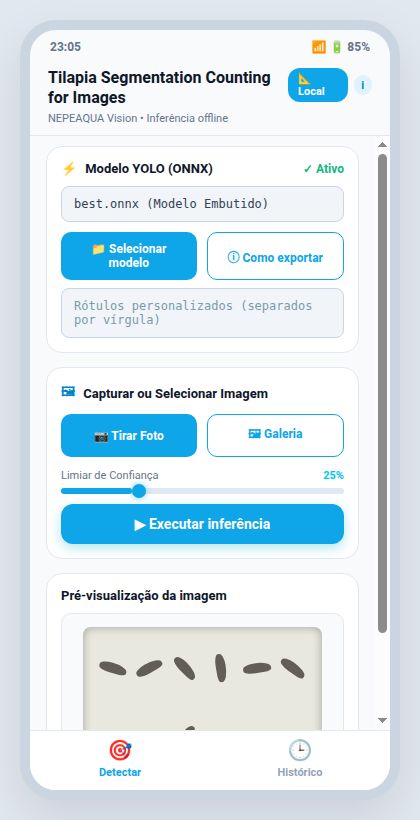
\includegraphics[width=\textwidth]{tela1.png}
    \caption{Tela 1: Configuração e Seleção de Imagem}
    \label{fig:tela1}
\end{subfigure}
\hfill
\begin{subfigure}[b]{0.46\textwidth}
    \centering
    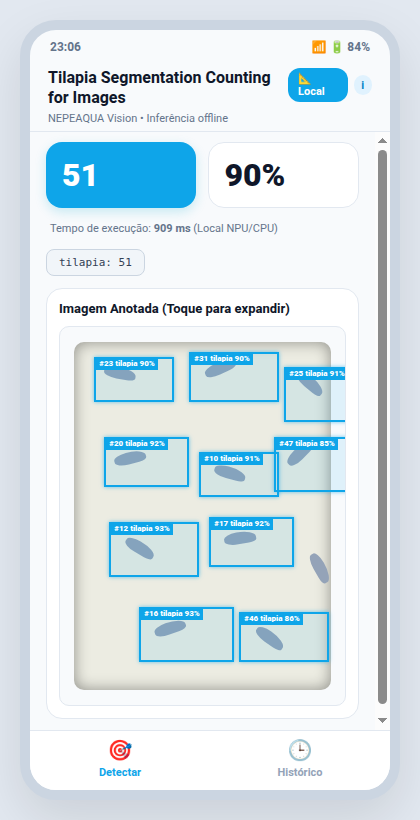
\includegraphics[width=\textwidth]{tela2.png}
    \caption{Tela 2: Resultados e Visualização Anotada}
    \label{fig:tela2}
\end{subfigure}
\caption{Protótipos para a execução da inferência e exibição direta das caixas anotadas.}
\label{fig:prototipos_execucao}
\end{figure}

\subsection{Telas de Histórico e Detalhamento das Caixas (Telas 3 e 4)}
As Figuras \ref{fig:tela3} e \ref{fig:tela4} ilustram o fluxo de consulta onde o usuário visualiza o histórico de análises e acessa os detalhes geométricos de cada caixa delimitadora.

\begin{figure}[htbp]
\centering
\begin{subfigure}[b]{0.46\textwidth}
    \centering
    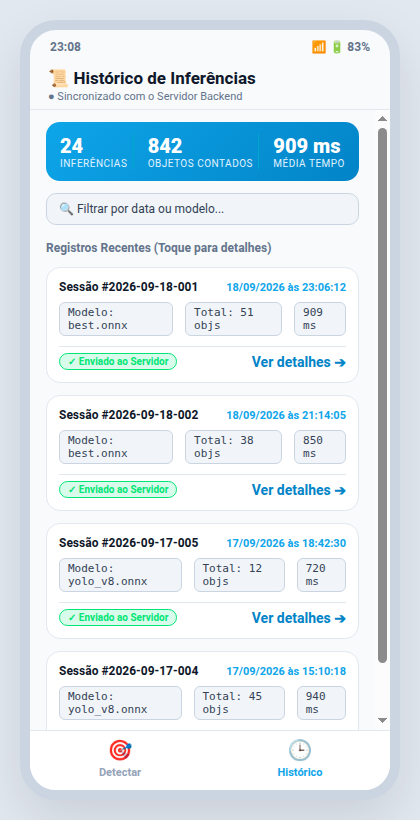
\includegraphics[width=\textwidth]{tela3.png}
    \caption{Tela 3: Histórico de Inferências (com Data e Hora)}
    \label{fig:tela3}
\end{subfigure}
\hfill
\begin{subfigure}[b]{0.46\textwidth}
    \centering
    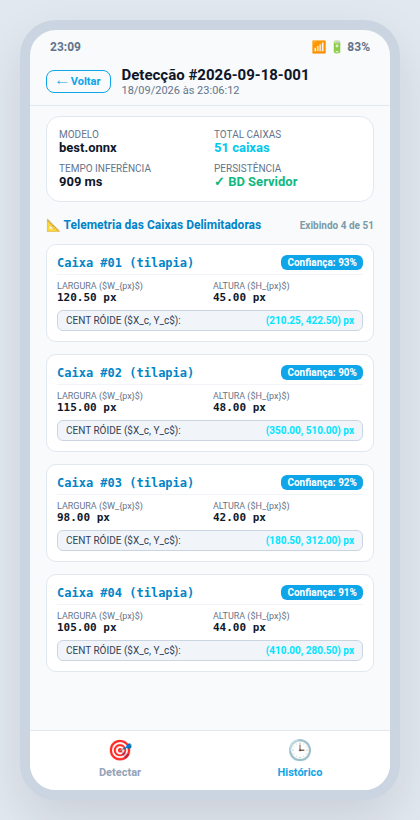
\includegraphics[width=\textwidth]{tela4.png}
    \caption{Tela 4: Detalhamento Geométrico das Caixas}
    \label{fig:tela4}
\end{subfigure}
\caption{Protótipos para o fluxo de histórico e consulta detalhada das caixas delimitadoras.}
\label{fig:prototipos_historico}
\end{figure}

---

\newpage
\section{Orientação para Criação do Design System e Telas}

\textbf{Os alunos deverão elaborar o seu próprio Design System}, podendo escolher a paleta de cores e tipografia. Contudo, \textbf{o aplicativo deve obrigatoriamente seguir o tema Light Mode e ser desenvolvido utilizando exclusivamente a biblioteca Jetpack Compose (não será aceito o uso de XML Views)}. 

Além disso, a estrutura de navegação deve contemplar uma \textbf{Bottom Navigation Bar} com os itens \textbf{Detectar} e \textbf{Histórico}, além das seguintes 4 telas:

\begin{enumerate}
    \item \textbf{Tela 1 (Configuração \& Entrada):} Escolha do modelo ONNX, opções de Câmera/Galeria e Slider de Limiar de Confiança.
    \item \textbf{Tela 2 (Resultado Gráfico):} Exibição da contagem total, tempo em $ms$ e imagem anotada com as caixas sobrepostas.
    \item \textbf{Tela 3 (Histórico de Inferências):} Listagem cronológica de todas as sessões de inferência salvas (exibindo data, hora, quantidade de objetos, modelo utilizado e indicador de envio ao servidor).
    \item \textbf{Tela 4 (Detalhamento Geométrico das Caixas):} Tela de consulta acionada ao tocar em um item da Tela 3, apresentando a auditoria individual de cada caixa delimitadora (\textit{Bounding Box}):
    \begin{itemize}
        \item Identificador da caixa (ex: \texttt{Caixa \#01}).
        \item Rótulo da classe e percentual de confiança.
        \item Dimensões exatas: Largura ($W_{px}$) e Altura ($H_{px}$) em pixels.
        \item Coordenadas exatas do Centróide ($X_{centroide}, Y_{centroide}$) em pixels.
        \item Área da caixa em pixels² ($A_{px}$).
    \end{itemize}
\end{enumerate}

---

\section{Critérios de Avaliação (Pontuação total: 10,0)}

\begin{table}[h!]
\centering
\begin{tabular}{p{11.5cm}c}
\toprule
\textbf{Critério de Avaliação} & \textbf{Pontuação} \\
\midrule
\textbf{1. Seleção do Dataset (Roboflow):} Escolha do problema, relevância e submissão prévia para aprovação do professor. & 1,0 pt \\
\midrule
\textbf{2. Design System e Interface Móvel:} Criação do Design System próprio e fidelidade à estrutura dos wireframes (Telas 1 a 4). & 2,0 pts \\
\midrule
\textbf{3. Inferência Local ONNX e Geometria:} Integração do modelo YOLO ONNX no Android e cálculo de largura, altura, centróides e área das caixas. & 2,5 pts \\
\midrule
\textbf{4. Fluxo de Histórico e Consulta (Telas 3 e 4):} Implementação da lista cronológica com data/hora e tela de detalhamento geométrico de cada caixa. & 2,0 pts \\
\midrule
\textbf{5. Servidor Backend, Persistência e Git:} API REST (Node/Python/Kotlin), persistência em BD/JSON e organização dos repositórios. & 1,5 pts \\
\bottomrule
\textbf{Total} & \textbf{10,0 pts} \\
\bottomrule
\end{tabular}
\end{table}

\vspace{0.3cm}

\section{Entrega e Informações Gerais}
\begin{itemize}
    \item \textbf{Formato:} Trabalho em grupo (até 4 alunos).
    \item \textbf{Submissão:} Links dos repositórios públicos no GitHub (Aplicativo Android + Servidor Backend) e arquivo APK até a data limite estipulada.
    \item \textbf{Linguagens:} \textbf{Kotlin com Jetpack Compose} para o aplicativo Android e linguagem livre para o Servidor Backend (Node.js, Python, Kotlin, etc.).
\end{itemize}

\end{document}
